\chapter{Implementation}

The design for the prototype I and prototype II detailed in the chapter \ref{DA} were implemented through iterative development process where the design for prototype I was drafted and implemented first, followed by the prototype II. This chapter details the procedure which was followed during the development and implementation of the thesis.  

\section{Current Cuttlefish Application} 
The native cuttlefish application is a 64-bit windows application, developed in C++ language using the Microsoft Visual Studio 12 SDK and the compiler used to build the code is Microsoft C/C++ V120 compiler. A project could be compiled either as static library or an executable in release or debug mode. The input for the application i.e. the path of the main configuration file, is presented a command line argument. The output generated by the application depends on the type of output component chosen in the component configuration. For each component, the behavior of the component is logged in the performance report and a log file for overall pipeline is written to the working directory at the end of the execution. This helps to analyze the component performance as well as to know the possible error by looking into the pipeline execution trace in case of a failure. Some of the projects of the application use external libraries (like zlib, little cms , poly2tri, boost, itk etc) which are either used as headers only or compiled for windows platform and linked as static library. 

Some parts of the computation performed by the application is on the GPU (graphics processing unit) and the code performing this computation is written and compiled using CUDA Toolkit. Another library used by the application is OpenGL(Open Graphics Library) wherein various powerful visualization features of the library are used for rendering, texture mapping etc. The minimum OpenGL version available to the application to run should be 2.0 as one of the APIs used- glCreateProgram, is available only in version 2.0 or higher. The native application has a strong dependency on availability of graphics library and CUDA.     

\section{Prerequisites for Distributed Cuttlefish Application Development} 

The goal of the thesis was earlier to provide a cloud service which could take the input from the user and do the computation using the cloud instances and provide the bitmaps as the output. With this goal, the native application had to be modified such that it could run on the cloud instances provided by the AWS (Amazon Web Services) as PAAS (Platform as a Service). The cluster of instances which formed the {\lq}cloud{\rq} were the basic Amazon EC2 instances which were virtual machines with Linux operating system. As the basic instances were virtual machine which were not GPU accelerated i.e. they did not have access to a GPU, the code which performed the GPU computing had to be changed such that only when the GPU is available, the code is compiled and used . So, this change to the native application code was done by creating a new configuration, other than release and debug, called as the CUDA\_FREE\_CONFIG which got rid of the dependency on availability of CUDA on the system running the application. The code performing the GPU computing is defined under if-defs to get the CUDA\_FREE\_CONFIG as seen in the Listing \ref{lst:CFC}

\begin{lstlisting}[language=C++,label={lst:CFC},caption={CUDA free configuration}]
//....
#ifndef CUDA_FREE	
			inline operator std::shared_ptr<VoxelSliceGPU>()
			{
				if (m_channel == m_invalidIndex)
					return nullptr;
				validate();
				return std::dynamic_pointer_cast<VoxelSliceGPU>(m_pContainer->m_slices[m_channel][m_slice]);
			}

#endif
//....
\end{lstlisting}

The CUDA\_FREE\_CONFIG configuration was still only for windows platform and the projects needed to be compiled such that they were compatible with Linux and it was necessary to get rid of the windows specific dependencies. To achieve portability and make the cross-platform build of the application possible, a configuration file called as the {\lq}CMakeLists.txt{\rq}  was written for each project of the application. Using CMake, an open-source system that manages the build process for an operating system in a compiler independent manner, all the project's cmakelists.txt files were parsed to generate the desired solution (depending on the generator chosen by the developer) i.e. the solution file could be Microsoft Visual Studio 12 solution or Unix makefiles or Eclipse CDT Unix makefiles. After using cmake to generate makefiles for linux system, the process to remove the windows specific code was started but could not be completed  due to time limitation (as it required rigorous amount changes). Hence, instead of using basic EC2 instances running Linux, a decision to use basic EC2 instances running windows operating system was made.    

The next step was to check if the CUDA free application configuration could run on an instance i.e. virtual machine with windows operating system. The application crashed in the call to the glCreateProgram api on the instance as the OpenGL version was 1.1. The fix for this issue would be to make OpenGL version 2.0 available on the instance i.e. the Virtual Machine. This cannot be done as OpenGL has a hardware limitation and the virtual machines use virtual GPUs which cannot support OpenGL 2.0 and provide support for only GPU basics. Hence, as most of the basic cloud instances (irrespective of the vendor/provider) are virtual machines supporting only GPU basics, the application could not be run on these instances. Therefore, instead of using a cloud of virtual machines as compute nodes, a decision to use physical processors as compute nodes was made, hence instead of cloud computing, cluster computing was chosen as the distributed system . 

The physical processors are 64-bit machines which run windows operating system and have access to the GPUs with the OpenGL 2.0 version available to the application. These physical machines are connected via the enterprise network. Though the compute nodes already had a common network, to use them as a cluster there was a need to perform a few installations to enable `clustering` which are detailed in the section \ref{ICS}. 


\section{Installation and Cluster Set-up} \label{ICS}

To begin with, a cluster with 2 nodes was created such that the nodes were connected to each other via a common network. To check if the cluster nodes could communicate, a simple ping test was performed. The next step was to write a program which performed a simple task in a distributed fashion and to run it on the cluster. For the cluster to work as system where the processing can be shared, there needs to be a way in which the cluster nodes can be named and the work to be done by each node could be distinguished i.e. assign roles to the nodes. There are many types of hardware/software solutions for the cluster which enable naming and role distinction among cluster nodes. The decision to use MPI-Message Passing Interface, was made to achieve naming and role assignment amongst the cluster nodes. MPI is the open standard specification for message passing libraries which provide apis to enable communication, role distinction and naming amongst the cluster nodes. There are various implementations of the specification available which basically perform the same thing i.e. message passing amongst the cluster nodes but are different with respect to the platform they support, commands to compile and launch the program, debugging and developed by different institutions. 
Some of the implementations are free-ware and some aren\textquotesingle t. As currently, cuttlefish is a windows application developed using Microsoft visual studio, the Microsoft\textquotesingle s implementation of MPI called as MSMPI is used. 

To use MSMPI, on each node of the cluster, the MS-MPI SDK is downloaded and installed. To verify if the installation and setup is done correctly, the environment variables are checked using the command {\lq} set MSMPI {\rq}. The environment variables which are particularly interesting are \$MSMPI\_INC\$, \$MSMPI\_BIN\$, and \$MSMPI\_LIB64\$. The table \ref{MSMPI-ENV} summarizes the details about these variable. 

\begin{table}[]
\centering
\label{my-label}
\begin{tabular}{|l|l|l|ll}
\cline{1-3}
\begin{tabular}[c]{@{}l@{}}Environment\\ Variable\end{tabular} & Value                                       & Significance                                 &  &  \\ \cline{1-3}
MSMPI\_INC                                                     & ..\textbackslash Microsoft SDKs\textbackslash MPI\textbackslash Include               & Path to find the headers                     &  &  \\ \cline{1-3}
MSMPI\_LIB64                                                   & ..\textbackslash Microsoft SDKs\textbackslash MPI\textbackslash Lib\textbackslash x64\textbackslash & Path to find the libraries for 64 bit system &  &  \\ \cline{1-3}
MSMPI\_BIN                                                     & ..\textbackslash Microsoft MPI\textbackslash Bin\textbackslash          & Path to find the binaries                    &  &  \\ \cline{1-3}
\end{tabular}
\label{MSMPI-ENV}
\caption{ MS-MPI Environment Variable}
\end{table}

To compile a program which will run on the cluster where the nodes communicate using MPI, the directories which help to resolve the reference to header files specific to MPI and path to the libraries which resolve linking to the MPI functions are incorporated in the project. Before running the program, a process management system which allows to manage the parallel processes on the cluster nodes should be executed on each of the cluster node. For MPI, the process management system used is called as SMPD (Simple Multipurpose Daemon) which is part of the software component of the process manager provided by Intel. It allows starting and managing parallel jobs on the cluster nodes. SMPD is used as a windows service and is set during the MPI installation. Ideally, the version of SMPD running on each node in the cluster should be same, although if there are different versions of SMPD, there is a possibility to disable the check for the versions. As the SMPD service is set during MPI installation, the version of SMPD is compatible with the mpiexec version. To run the program, mpiexec command is used with the arguments specifying the number of hosts, host names, the directory where the executable for application to be launched is available, the name of the executable followed by arguments to the executable. The listing \ref{lst:MPIC} is an example of the command syntax to launch the application using mpiexec command.  

\begin{lstlisting}[language=C++,label={lst:MPIC},caption={mpiexec syntax}]
mpiexec -hosts 2 PC2215 PC2286 -wdir \\pc2215\bin\Release\ Cuttlefish.exe \\pc2215\main\_conf.json
\end{lstlisting}  
	
\section{Introduction to New Components}

After the set-up of the required software, the next step was implementation of the prototype I followed by the implementation of prototype II. The components of both the prototypes are discussed in detail in the chapter \ref{DA}. Each of the new component is inherited from the class called as the \textit{PrintingComponent} and is registered using the component name. During the creation of the pipeline i.e. when the component configuration is parsed, each of the component is created and initialized with the required parameter values. The parameter values for each component are set in the configuration file. The Figure \ref{fig:Componentdiagram} summarizes the new components(underlined component names) introduced during the implementation of the thesis.

\begin{figure}[ht!]
\centering
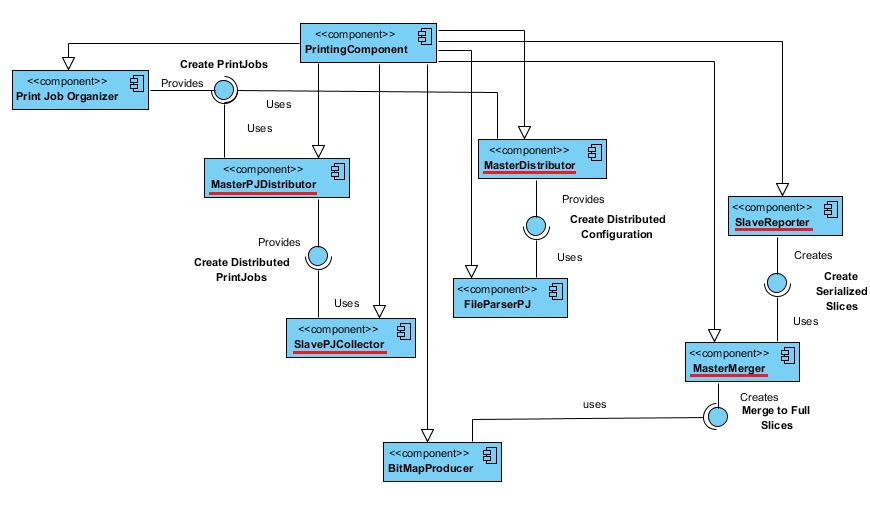
\includegraphics[scale=0.8]{Componentdiagram.PNG}
\caption{Component Diagram For New Components}
\label{fig:Componentdiagram}
\end{figure}

Each component has an input it receives from another component and an output that it generates which may be used by the following component in the pipeline(if any). The dependency is depicted in the Figure \ref{fig:Componentdiagram} by the {\lq}lollipop{\rq} symbol where in the half circle depicts interface exported by the component and the circle represents the interface that is imported by the component, for example, the component \textit{MasterDistributorPJ}uses the print job created by the \textit{PrintJobOrganizer} and provides the print jobs with distributed print objects used by the \textit{SlavePJCollector}.

The new classes which were implemented during the thesis are enlisted in the Table \ref{CSPI} for prototype I, in the Table \ref{CSPII} for prototype II and common classes used by both the prototypes are listed in Table \ref{ComClass}. 

\begin{table}[]
\centering
\caption{Class specific for Prototype I}
\label{CSPI}
\begin{tabular}{|l|l|l}
\cline{1-2}
\textbf{Class}              & 
\textbf{Purpose}                                                                                                                                                                                                &  \\ \cline{1-2}
MasterDistributor & \begin{tabular}[c]{@{}l@{}}Class for slave work item creation and distribution. \\ The work item created is the main configuration file \\ containing the assigned number of print object files.\end{tabular} &  \\ \cline{1-2}
\end{tabular}
\end{table}



\begin{table}[]
\centering
\caption{Classes specific for Prototype II}
\label{CSPII}
\begin{tabular}{|l|l|l}
\cline{1-2}
\textbf{Class}      & \textbf{Purpose}                                                                                                                                                                   &  \\ \cline{1-2}
MasterPJDistributor & \begin{tabular}[c]{@{}l@{}}Class for creation of print jobs with the print objects \\ distributed using the cost function and \\ serialization of the print jobs\end{tabular}      &  \\ \cline{1-2}
SlavePJCollector    & \begin{tabular}[c]{@{}l@{}}Class for collection of the serialized print job, \\ de-serialization of the print jobs and loading\\ the texture data to the node memory.\end{tabular} &  \\ \cline{1-2}
\end{tabular}
\end{table}


\begin{table}[]
\centering
\caption{Common Classes For Prototype I and II}
\label{ComClass}
\begin{tabular}{|l|l|l}
\cline{1-2}
\textbf{Class}                & \textbf{Purpose}                                                                                                                                                           &  \\ \cline{1-2}
MasterPrintingSoftware        & Creates and manages the printing software for the master node                                                                                                              &  \\ \cline{1-2}
SlavePrintingSoftware         & Creates and manages the printing software for the slave node                                                                                                               &  \\ \cline{1-2}
P3DNetworkComm                & Interface exposing the methods for communication                                                                                                                           &  \\ \cline{1-2}
P3dNetworkCommMPI             & \begin{tabular}[c]{@{}l@{}}Implements the interface methods using MPI as \\ the message passing library\end{tabular}                                                       &  \\ \cline{1-2}
DistributedComponentParser    & Parser for the JSON files used for distributed computing                                                                                                                   &  \\ \cline{1-2}
DistributedComponentInitiator & \begin{tabular}[c]{@{}l@{}}Initiator class for distributed computing. It manages \\ the cluster creation, execution and shut down of the\\ printing software\end{tabular}  &  \\ \cline{1-2}
SyncVoxelSlicesContainer      & \begin{tabular}[c]{@{}l@{}}Synchronized voxel slice container allowing \\ synchronous access to multiple threads\end{tabular}                                              &  \\ \cline{1-2}
MasterMergerWorker            & \begin{tabular}[c]{@{}l@{}}Interface exposing methods for performing \\ collection of metadata, de-serialization and\\  writing partial slices to full slices\end{tabular} &  \\ \cline{1-2}
MasterMergerWorkerImpl        & \begin{tabular}[c]{@{}l@{}}Implementation of the MasterMergerWorker class \\ with a thread per slave\end{tabular}                                                          &  \\ \cline{1-2}
DistributedCostFunction       & \begin{tabular}[c]{@{}l@{}}Class for calculation of the threshold and cost \\ function used for load distribution\end{tabular}                                             &  \\ \cline{1-2}
SlaveReporter                 & \begin{tabular}[c]{@{}l@{}}Class which performs serialization of the slices \\ and reports them to master\end{tabular}                                                     &  \\ \cline{1-2}
MasterMerger                  & \begin{tabular}[c]{@{}l@{}}Class performing collection of partial slices \\ and generation of merged full slices\end{tabular}                                              &  \\ \cline{1-2}
SlaveDataBuffer               & Synchronous queue used by the thread of slave reporter class                                                                                                               &  \\ \cline{1-2}
\end{tabular}
\end{table}

\section{Communication Specifics}
\section{External Libraries}
\section{Debugging}
\section{Project Management}